\chapter{The Adjoint for Dynamical Systems}

\begin{flushright}
\textit{To understand the effect of an outcome, trace its influence backward through time.}

\medskip
\textit{The forward model tells you where you end up.\\
The adjoint tells you how you got there.}
\end{flushright}

\bigskip

Climate models routinely have 500 or more tunable parameters.
Forward sensitivity analysis using the FSE approach requires
one ODE solve per parameter: 500~solves on a modern workstation,
each taking 6~hours. Total: 3{,}000~hours, or 125~days.

The adjoint approach requires exactly two ODE solves: one forward,
one backward. Total: 12~hours.

The mathematics behind this 125-to-1 speedup is a direct extension
of the matrix adjoint from Chapter~5. In that chapter, the key operation
was transposing the coefficient matrix: $A \to A^T$. Here, the key
operation is transposing the differential operator, which turns a forward
ODE into a backward ODE. This chapter derives that operation step by step,
explains in plain language why the backward direction arises,
and implements the full calculation for the SIR epidemic model.
The notation is one step heavier than Chapter~5 --- integration by parts
and continuous-time functionals replace matrix transposes --- but the
underlying idea is the same transposition argument in a new space.
The adjoint sensitivity equations for ODE systems, including their
software implementation, are treated in depth by Cao et al.~\cite{cao2002adjoint};
a recent comparison of forward and adjoint methods on biological models is
given by Mester et al.~\cite{mester2022differential}.

%%------------------------------------------------------------
\section{The Timeline Figure}\index{adjoint method!backward in time}
\label{sec:timeline}
%%------------------------------------------------------------

The most important idea in this chapter: the reason the adjoint ODE
runs backward, is captured in Figure~\ref{fig:timeline} before any
equations appear.

\begin{figure}[htb]
\centering
\begin{tikzpicture}[
  thick,
  arr/.style={-{Latex[length=3.5mm]}, thick},
  darr/.style={-{Latex[length=3.5mm]}, thick, dashed},
]

%% Time axis
\draw[arr] (-0.3,0) -- (9.8,0) node[right]{$t$};
\node[below] at (0,0) {$0$};
\node[below] at (9.3,0) {$T$};
\draw (0,-0.08) -- (0,0.08);
\draw (9.3,-0.08) -- (9.3,0.08);

%% Forward ODE arrow
\draw[arr, very thick] (0,0.9) -- (9.3,0.9);
\node[above] at (4.65,0.9) {Forward ODE: state $\vec{u}(t)$};
\node[above, font=\small] at (4.65,0.5)
  {initial condition $\vec{u}(0) = \vec{u}_0$ at $t=0$};

%% Adjoint ODE arrow (backward)
\draw[darr, very thick] (9.3,-0.9) -- (0,-0.9);
\node[below] at (4.65,-0.9) {Adjoint ODE: $\lambda(t)$};
\node[below, font=\small] at (4.65,-1.3)
  {terminal condition $\lambda(T)$ at $t=T$};

%% Annotations
\node[left, align=right, font=\small] at (-0.3, 0.9)
  {propagates\\forward $\to$};
\node[right, align=left, font=\small] at (9.5,-0.9)
  {$\leftarrow$ propagates\\backward};

%% Brace for J
\draw[decorate, decoration={brace,amplitude=5pt}]
  (9.5, 0.05) -- (9.5, -0.05);
\node[right, font=\small, align=left] at (9.65, 0)
  {response\\$J$};

\end{tikzpicture}
\caption{The timeline for forward and adjoint sensitivity analysis.
         The forward ODE propagates the model state $\vec{u}(t)$ from
         the initial condition at $t=0$ toward the response $J$ at $t=T$.
         The adjoint ODE propagates the sensitivity weight $\lambda(t)$
         backward from a terminal condition at $t=T$, in the direction
         opposite to the forward problem.
         The two ODEs are not independent: the adjoint coefficient
         depends on the forward solution $\vec{u}(t)$ at every time step.}
\label{fig:timeline}
\end{figure}

The forward ODE begins at $t=0$ and moves right, building up the state
$\vec{u}(t)$ until it reaches the response $J$ at time $T$.
The adjoint ODE begins at $t=T$ and moves left, distributing the
response backward through time.

This opposite direction is not a numerical trick. It is a mathematical
necessity, explained in Section~\ref{sec:whybackward}.

%%------------------------------------------------------------
\section{Why Backward? Intuition Before Derivation}
\label{sec:whybackward}
%%------------------------------------------------------------

The adjoint ODE runs backward because the question it answers
is naturally backward: how much did each moment in time contribute
to the final value of $J$?

Think of the epidemic. A perturbation applied to the infectious
compartment at $t = 0$ has the entire simulation period to propagate:
it changes the dynamics at $t = 1$, $t = 2$, and all the way to $T$.
Its influence on $J$ is large. A perturbation applied at $t = T-\epsilon$
has almost no time to propagate before the simulation ends.
Its influence on $J$ is negligible.

So the ``weight'' we should assign to perturbations decreases
as we move from left to right along the time axis,
and increases as we move from right to left.
The adjoint variable $\lambda(t)$ is precisely this weight:
$\lambda(t)$ measures how sensitive the response $J$ is to
a perturbation of the state at time $t$.

At $t = T$, the weight is determined by the response functional
(how does $J$ change if the final state changes?).
At earlier times, $\lambda(t)$ is computed by propagating this
weight backward, accounting for how perturbations at time $t$
have time to amplify before reaching $T$.

The adjoint variable is large near $t = 0$ and small near $t = T$.
The adjoint ODE starts at the only time where we know $\lambda$
directly at $t = T$, and integrates backward to find
$\lambda(t)$ at all earlier times.

This must be understood before the derivation. The backward
direction of the adjoint is not a consequence of the algebra;
the algebra is a consequence of this backward structure.

The adjoint and forward problems are not independent:
the coefficient in the adjoint ODE at every time $t$ involves
$\vec{u}(t)$, the forward solution. The adjoint can only be
solved after the forward problem is solved and $\vec{u}(t)$
is stored at every time point needed.

\begin{selfcheck}
Suppose the response functional is $J = S(T)$ (the susceptible
population at the final time) and the epidemic has a peak at $t = 30$
in a 90-day simulation. At which time ($t = 5$, $t = 30$, or $t = 80$
would you expect $\lambda_I(t)$ to be largest in magnitude?
Explain without any calculation.
\end{selfcheck}
\begin{scAnswer}
$\lambda_I(t)$ at time $t$ measures how sensitive $J = S(T)$ is to a
perturbation of $I$ at time $t$. A perturbation to $I$ at $t = 5$
has 85~days to propagate and affect $S(90)$: a large window
of time for the perturbation to alter the epidemic trajectory.
A perturbation at $t = 80$ has only 10~days.
So $\lambda_I(t)$ should be largest at $t = 5$.
\end{scAnswer}

%%------------------------------------------------------------
\section{The Lagrange Multiplier Derivation}\index{Lagrange multiplier}\index{adjoint method!ODE derivation}
\label{sec:lagrange}
%%------------------------------------------------------------

\subsection{A Warm-Up: Exponential Decay}

Before the five-step derivation, work through the simplest possible case
to see exactly what the adjoint ODE looks like and how it gives the answer.

Let $\dot{u} = -pu$ with $u(0) = 1$ and $J = u(T)$.
The forward solution is $u(t) = e^{-pt}$, so $J = e^{-pT}$ and
$dJ/dp = -T e^{-pT}$ (by direct differentiation --- the ``correct'' answer).

The adjoint approach finds the same result differently.
For $F(u;p) = -pu$ and $g = 0$, $h(u) = u$:
\begin{itemize}[nosep]
  \item Adjoint ODE: $-\dot{\lambda} = F_u\,\lambda = -p\lambda$,
        so $\dot{\lambda} = p\lambda$.
  \item Terminal condition: $\lambda(T) = -h'(u(T)) = -1$.
  \item Solution (running backward from $T$): $\lambda(t) = -e^{p(t-T)}$.
  \item Sensitivity formula: $dJ/dp = -\int_0^T \lambda(t)\,F_p\,dt
        = -\int_0^T (-e^{p(t-T)})(-u(t))\,dt
        = -\int_0^T e^{p(t-T)}e^{-pt}\,dt
        = -\int_0^T e^{-pT}\,dt = -Te^{-pT}$. \checkmark
\end{itemize}
The adjoint gave the same derivative using only two ODE solves (forward,
then backward), with no dependence on $m$ (how many parameters there are).
If $p$ were joined by 49 other parameters, the cost would still be
two ODE solves plus 49 integrals.

Now we derive this procedure in full generality.

\subsection{The Five-Step Derivation}

The derivation proceeds through five numbered steps, each announced
before it is executed. The scalar ODE case is treated fully; the
vector case follows by replacing scalars with vectors and matrices.

\subsection{Setup}

Consider the initial value problem
\begin{equation}
  \dot{u} = F(u; p), \qquad u(0) = u_0,
  \label{eq:fwd_ode}
\end{equation}
with a response functional
\begin{equation}
  J = \int_0^T g(u; p)\,dt + h(u(T)).
  \label{eq:functional}
\end{equation}
Here $g$ is the running cost (an integrand depending on the solution
and parameters) and $h$ is a terminal cost (depending only on the
final state). We want $dJ/dp$ without solving the FSE.

\medskip

The strategy is identical to Chapter~5: introduce an auxiliary variable,
choose it to cancel the unknown sensitivity $\partial u/\partial p$,
and read off the result from what remains.
In Chapter~5 the auxiliary variable was a vector $\vec{v}$ satisfying
$A^T\vec{v} = \vec{c}$; here it is a function $\lambda(t)$ satisfying
a backward ODE.

\medskip
\textbf{Step 1: Introduce the Lagrange multiplier.}

We introduce an auxiliary function $\lambda(t)$, called
the adjoint variable or Lagrange multiplier, and observe that,
because $u(t)$ satisfies the ODE~\eqref{eq:fwd_ode}:
\[
  \int_0^T \lambda(t)\bigl[\dot{u} - F(u;p)\bigr]\,dt = 0.
\]
This is the ODE constraint written as a vanishing integral.
Define the augmented functional
\begin{equation}
  \tilde{J} = J + \int_0^T \lambda(t)\bigl[\dot{u} - F(u;p)\bigr]\,dt.
  \label{eq:augmented}
\end{equation}
Since the bracketed term is zero, $\tilde{J} = J$.
The strategy, carried over from Chapter~5, is to choose
$\lambda(t)$ so that $\partial u/\partial p$ disappears when we
differentiate $\tilde{J}$ with respect to $p$.

\medskip\noindent\textit{Physical analogy.}
Think of a building inspector who records the strain in each beam throughout the day.
The inspector's record is $\lambda(t)$: it does not change the building,
but it carries a running account of how much each moment in time contributes to
the structure's overall stress $J$.
Adding the constraint integral is like attaching a running tally that is identically
zero as long as the beams obey the equilibrium equations --- it costs nothing,
but it opens the door to measuring sensitivity.

\medskip
\textbf{Step 2: Differentiate with respect to $p$.}

Denote $w = \partial u/\partial p$. Differentiating~\eqref{eq:augmented}:
\begin{equation}
  \dd{\tilde{J}}{p}
  = \int_0^T g_u\,w\,dt + h'(u(T))\,w(T)
    + \int_0^T \lambda\bigl[\dot{w} - F_u\,w - F_p\bigr]\,dt.
  \label{eq:dJtilde}
\end{equation}
The unknown $w = \partial u/\partial p$ appears in three places.
The next step eliminates it by choosing $\lambda$ appropriately.

\medskip\noindent\textit{Physical analogy.}
Differentiating with respect to $p$ is like asking: if we nudge a design parameter ---
say, the stiffness of one beam --- how does the overall stress $J$ respond?
The sensitivity $w = \partial u/\partial p$ represents the ripple that nudge sends
through the entire structure over time. It appears everywhere because the system
is coupled; $\lambda(t)$ will be chosen precisely to absorb those ripples.

\medskip
\textbf{Step 3: Integrate by parts.}

The term $\int_0^T \lambda \dot{w}\,dt$ contains $\dot{w}$.
We remove the time derivative from $w$ by integrating by parts:
this is the key step, and it is the ODE analog of the matrix
transposition $v^T A = (A^T v)^T$ in Chapter~5.

\begin{equation}
  \int_0^T \lambda\,\dot{w}\,dt
  = \bigl[\lambda\,w\bigr]_0^T - \int_0^T \dot{\lambda}\,w\,dt
  = \lambda(T)\,w(T) - \lambda(0)\,w(0) - \int_0^T \dot{\lambda}\,w\,dt.
  \label{eq:IBP}
\end{equation}
Substituting into~\eqref{eq:dJtilde}:
\begin{align}
  \dd{\tilde{J}}{p}
  &= \int_0^T g_u\,w\,dt + h'(u(T))\,w(T) \notag\\
  &\quad + \lambda(T)\,w(T) - \lambda(0)\,w(0)
    - \int_0^T \dot{\lambda}\,w\,dt
    - \int_0^T \lambda\,F_u\,w\,dt
    - \int_0^T \lambda\,F_p\,dt.
  \label{eq:dJfull}
\end{align}
Collecting the $w$-terms (the terms involving the unknown sensitivity):
\begin{equation}
  \dd{\tilde{J}}{p}
  = \underbrace{\bigl[h'(u(T)) + \lambda(T)\bigr]w(T)
    - \lambda(0)\,w(0)
    + \int_0^T \bigl[g_u - \dot{\lambda} - \lambda F_u\bigr]w\,dt}_{%
    \text{terms involving } w = \partial u/\partial p}
    - \int_0^T \lambda\,F_p\,dt.
  \label{eq:dJcollected}
\end{equation}

Integration by parts is not merely an algebraic trick.
It is exactly the operation that moves the time derivative
from $w$ to $\lambda$, transforming the FSE into
the adjoint ODE, just as matrix transposition moved
the linear operator from $u$ to $v$ in Chapter~5.

\medskip\noindent\textit{Physical analogy.}
Think of two runners passing a baton around a track.
Forward mode carries $\dot{w}$ --- the baton is held by the sensitivity variable.
Integration by parts hands the baton to $\lambda$: now $\dot{\lambda}$ carries
the time derivative instead, and $w$ appears without any derivative.
This exchange is what makes it possible to choose $\lambda$ to cancel $w$
in the next step; without it, we could not get rid of $\dot{w}$ by specifying
an ODE for $\lambda$ alone.

\medskip
\textbf{Step 4: Choose $\lambda$ to eliminate $w$.}

For the sensitivity formula~\eqref{eq:dJcollected} to be
free of $w$, the coefficient of $w$ must vanish everywhere.
This requires three conditions to hold simultaneously.

First, the integrand coefficient of $w(t)$ must vanish for all $t \in (0,T)$:
\begin{equation}
  -\dot{\lambda} - \lambda F_u + g_u = 0,
  \quad\text{i.e.,}\quad
  \dot{\lambda} = -F_u\,\lambda + g_u.
  \label{eq:adj_wrong_sign}
\end{equation}
Written in standard form (with the sign convention consistent
with backward integration):
\begin{equation}
  \boxed{-\dot{\lambda} = F_u\,\lambda - g_u.}
  \label{eq:adjODE}
\end{equation}
Second, the coefficient of $w(T)$ must vanish:
\begin{equation}
  h'(u(T)) + \lambda(T) = 0,
  \quad\text{i.e.,}\quad
  \lambda(T) = -h'(u(T)).
  \label{eq:termcond}
\end{equation}
Third, the term $\lambda(0)w(0)$ must vanish. Since $u(0) = u_0$
does not depend on $p$, we have $w(0) = \partial u_0/\partial p = 0$,
so this term vanishes automatically.

The terminal condition~\eqref{eq:termcond} does not arise because
we are running the ODE backward. It arises because the response
functional involves the final state $h(u(T))$, and differentiating
this with respect to $p$ produces a boundary term at $t = T$.
This is a fundamental distinction: the terminal condition is imposed
by the response functional, not by the direction of integration.

\medskip\noindent\textit{Physical analogy.}
Choosing $\lambda$ to kill every $w$-term is like tuning the damping in a bridge
so that any vibration induced by a parameter perturbation is immediately cancelled.
The terminal condition $\lambda(T) = -h'(u(T))$ is the inspector's final reading:
at the end of the day the ledger must close, recording exactly how sensitive the
last measured outcome is to the final state. Once $\lambda(t)$ is tuned,
$w$ has nowhere to appear in the sensitivity formula --- it has been designed out.

\medskip
\textbf{Step 5: Read off the sensitivity formula.}

With $\lambda(t)$ satisfying~\eqref{eq:adjODE}--\eqref{eq:termcond},
all terms involving $w$ in~\eqref{eq:dJcollected} vanish and:
\begin{equation}
  \boxed{\dd{J}{p} = -\int_0^T \lambda(t)\,F_p(u(t);p)\,dt
                     - \lambda(0)\,\dd{u_0}{p}.}
  \label{eq:sensfml}
\end{equation}
When the initial condition does not depend on $p$, the second term
vanishes. The sensitivity with respect to any parameter $p_j$ is then:
\begin{equation}
  \dd{J}{p_j} = -\int_0^T \lambda(t)\,\pd{F}{p_j}\,dt.
  \label{eq:sensfml_simple}
\end{equation}
One backward ODE solve for $\lambda(t)$ gives all $m$ sensitivities
via $m$ scalar integrals, exactly the cost advantage we sought.

\medskip\noindent\textit{Physical analogy.}
The inspector's record $\lambda(t)$ is now complete: one backward sweep through
time, consulting the forward solution $u(t)$ at each moment, accumulates
everything needed. Reading off $dJ/dp_j$ is then as simple as computing a
running total --- one scalar integral per parameter, with no additional solves.
The backward sweep is the price paid once; the $m$ integrals are the
dividend collected once for every parameter in the model.

\subsection{The Vector Case}

For the vector system $\dot{\vec{u}} = \vec{F}(\vec{u}; \vec{p})$
with $\vec{u} \in \R^n$ and functional
$J = \int_0^T g(\vec{u};\vec{p})\,dt + h(\vec{u}(T))$,
the derivation is identical with scalars replaced by vectors
and $F_u$ replaced by the Jacobian $J_F = \partial\vec{F}/\partial\vec{u}$.
The adjoint ODE and terminal condition become:
\begin{align}
  -\dot{\vec{\lambda}} &= J_F^T\,\vec{\lambda} - \nabla_u g^T,
  \label{eq:adj_vec} \\
  \vec{\lambda}(T) &= -\nabla_u h^T\big|_{t=T}.
  \label{eq:tc_vec}
\end{align}

\noindent\textbf{Linearity of the adjoint ODE.}
Just as Theorem~\ref{thm:linearFSE} showed that the FSE is always
linear in the forward sensitivity variable $\partial\vec{u}/\partial p_j$,
the adjoint ODE is always linear in $\vec{\lambda}(t)$ ---
even when the forward ODE is nonlinear in $\vec{u}(t)$.
The coefficient $J_F^T(\vec{u}(t))$ is a matrix that depends on the
forward solution, but not on $\vec{\lambda}$ itself.
This linearity is the ODE counterpart of the algebraic linearity
from Chapter~5, and it is why the adjoint is tractable: regardless
of how complex the forward dynamics are, the adjoint ODE is a
linear ODE that can be solved efficiently.

\medskip\noindent
\textbf{Sign convention.}
We write the adjoint in backward-time form as $-\dot{\vec{\lambda}} = \ldots$
to match the MATLAB implementation: \texttt{ode45} with \texttt{tspan = [T, 0]}
integrates backward automatically.
In the sensitivity formula~\eqref{eq:sensfml_vec},
the minus sign is already absorbed: no additional sign change is needed
when reading off $dJ/dp_j$ from the integral.

The sensitivity formula becomes:
\begin{equation}
  \dd{J}{p_j} = -\int_0^T \vec{\lambda}^T\,\pd{\vec{F}}{p_j}\,dt
               - \vec{\lambda}(0)^T\,\pd{\vec{u}_0}{p_j}.
  \label{eq:sensfml_vec}
\end{equation}

\unifyingidea{2} The derivation is now complete, and this is Unifying Idea~2 in its full generality.
The adjoint in Chapter~5 was $A^T\vec{v} = \vec{c}$:
the transposed coefficient matrix $A^T$ applied to $\vec{v}$.
The adjoint here is $-\dot{\vec{\lambda}} = J_F^T\vec{\lambda} - \nabla_u g^T$:
the transposed Jacobian $J_F^T$ applied to $\vec{\lambda}$, with
the sign reversal arising from the integration by parts~\eqref{eq:IBP}.
The integration by parts is the exact functional-analytic analog
of the matrix transposition $A \to A^T$ from Chapter~5.
Appendix~\ref{appsec:IBP} makes this analogy precise through the
Lagrange identity, and Appendix~\ref{appsec:lagrange} derives
the sensitivity formula~\eqref{eq:sensfml_vec} rigorously from it.
The terminal condition~\eqref{eq:tc_vec} is the time-dependent
analog of the right-hand side $\vec{c}$ in $A^T\vec{v} = \vec{c}$.
This is one idea.

\begin{selfcheck}
For the scalar ODE $\dot{u} = -pu$ with $J = u(T)$
(no running cost, $g = 0$, $h(u) = u$):
(a) Write the adjoint ODE and terminal condition using
    equations~\eqref{eq:adjODE} and~\eqref{eq:termcond}.
(b) Solve the adjoint ODE analytically.
(c) Use formula~\eqref{eq:sensfml_simple} to compute $dJ/dp$.
(d) Verify by solving the forward ODE analytically and differentiating.
\end{selfcheck}
\begin{scAnswer}
(a) $F = -pu$, so $F_u = -p$.
Adjoint ODE: $-\dot{\lambda} = -p\lambda$, i.e., $\dot{\lambda} = p\lambda$.
Terminal condition: $\lambda(T) = -h'(u(T)) = -1$.

(b) $\dot{\lambda} = p\lambda$ with $\lambda(T) = -1$.
Integrating forward from $T$ (backward in time):
$\lambda(t) = -e^{p(t-T)}$.

(c) $F_p = -u$. Sensitivity formula:
$dJ/dp = -\int_0^T \lambda(t)(-u(t))\,dt = \int_0^T \lambda(t)u(t)\,dt$.
The forward solution is $u(t) = u_0 e^{-pt}$.
$dJ/dp = \int_0^T (-e^{p(t-T)})(u_0 e^{-pt})\,dt
= -u_0 e^{-pT}\int_0^T dt = -u_0 T e^{-pT}$.

(d) $J = u(T) = u_0 e^{-pT}$, so $dJ/dp = -u_0 T e^{-pT}$. \checkmark
\end{scAnswer}

%%------------------------------------------------------------
\section{The SIR Model --- Full Adjoint Treatment}
\label{sec:sirAdjoint}
%%------------------------------------------------------------

We apply the derivation to the SIR model, writing all adjoint equations
explicitly and implementing the full calculation in MATLAB.

\subsection{Setup and Response Functional}

The SIR model~(4.4)--(4.6) with interpretable \POIs
$\vec{p} = (k, \beta, \tau, L)$:
\begin{align*}
  F_S &= \mu N - \frac{k\beta SI}{N} - \mu S, \\
  F_I &= \frac{k\beta SI}{N} - (\gamma + \mu)I, \\
  F_R &= \gamma I - \mu R,
\end{align*}
where $\gamma = 1/\tau$ and $\mu = 1/L$.
The response functional is
\begin{equation}
  J = \int_0^T I(t)\,dt,
  \label{eq:sirJ}
\end{equation}
the total number of infectious person-days: a measure of
the total disease burden. Here $g(\vec{u}) = I$, $h = 0$.

\subsection{The Jacobian}

The Jacobian $J_F = \partial(F_S, F_I, F_R)/\partial(S, I, R)$ evaluated
at the forward solution $(S(t), I(t), R(t))$:
\begin{equation}
  J_F =
  \begin{pmatrix}
    -\dfrac{k\beta I}{N} - \mu & -\dfrac{k\beta S}{N} & 0 \\[8pt]
     \dfrac{k\beta I}{N} & \dfrac{k\beta S}{N} - \gamma - \mu & 0 \\[8pt]
    0 & \gamma & -\mu
  \end{pmatrix}.
  \label{eq:sirJacobian}
\end{equation}

\subsection{Adjoint ODEs}

With $g_S = 0$, $g_I = 1$, $g_R = 0$ (since $g = I$),
the adjoint system $-\dot{\vec{\lambda}} = J_F^T\vec{\lambda} - \nabla g^T$
written out fully is:
\begin{align}
  -\dot{\lambda}_S &= \left(-\frac{k\beta I}{N} - \mu\right)\lambda_S
                     + \frac{k\beta I}{N}\,\lambda_I, \label{eq:adj_S}\\[4pt]
  -\dot{\lambda}_I &= -\frac{k\beta S}{N}\,\lambda_S
                     + \left(\frac{k\beta S}{N} - \gamma - \mu\right)\lambda_I
                     + \gamma\lambda_R - 1, \label{eq:adj_I}\\[4pt]
  -\dot{\lambda}_R &= -\mu\lambda_R. \label{eq:adj_R}
\end{align}
Terminal conditions (since $h = 0$):
\begin{equation}
  \lambda_S(T) = \lambda_I(T) = \lambda_R(T) = 0.
  \label{eq:sirTC}
\end{equation}
These three ODEs are integrated backward from $t=T$ to $t=0$,
using the stored forward solution $(S(t), I(t), R(t))$
to evaluate the time-varying coefficients.

\subsection{Sensitivity Formulas}

For each \POI, the sensitivity is the integral~\eqref{eq:sensfml_vec}
evaluated using the stored $\vec{\lambda}(t)$:
\begin{align}
  \dd{J}{\beta} &= -\int_0^T \frac{kSI}{N}(\lambda_I - \lambda_S)\,dt,
  \label{eq:dJdbeta}\\[4pt]
  \dd{J}{k}     &= -\int_0^T \frac{\beta SI}{N}(\lambda_I - \lambda_S)\,dt,
  \label{eq:dJdk}\\[4pt]
  \dd{J}{\tau}  &= -\int_0^T \pd{F_I}{\tau}\,\lambda_I\,dt
                 = -\int_0^T \frac{1}{\tau^2}\,I\,\lambda_I\,dt,
  \label{eq:dJdtau}\\[4pt]
  \dd{J}{L}     &= -\int_0^T \left[\pd{F_S}{L}\lambda_S
                               + \pd{F_I}{L}\lambda_I
                               + \pd{F_R}{L}\lambda_R\right]dt.
  \label{eq:dJdL}
\end{align}
Normalized sensitivity indices follow from Definition~2.1:
$\SI{p_j}{J} = (p_j/J)(dJ/dp_j)$.

\medskip\noindent
\textbf{Multiple QOIs and correlated outputs.}
When the study involves $r > 1$ response functionals
--- for example, both $J_1 = \int_0^T I\,dt$ (total burden)
and $J_2 = \max_t I(t)$ (peak infections) ---
the adjoint is solved once per \QOI, giving $r$ backward solutions
$\vec{\lambda}^{(1)}(t), \ldots, \vec{\lambda}^{(r)}(t)$.
Even when the \POIs are independent (uncorrelated inputs),
the \QOIs are almost always correlated outputs: both $J_1$ and $J_2$
depend on the same forward trajectory $\vec{u}(t)$,
so any parameter change affects both simultaneously.
This correlation among outputs is handled automatically by the adjoint.
Each backward solve $\vec{\lambda}^{(k)}$ captures the full sensitivity
of $J_k$ to perturbations of the shared state, without any special
treatment of the output correlation.
The user does not model or correct for QOI correlation ---
the adjoint naturally produces consistent, correct sensitivities
for all $r$ response functionals by virtue of working through
the same forward trajectory.

\subsection{The Adjoint Variable and Its Interpretation}

Figure~\ref{fig:sir_lambdaI} shows $I(t)$ and $\lambda_I(t)$ computed
for nominal parameter values over a 90-day simulation.

\begin{figure}[htb]
\centering
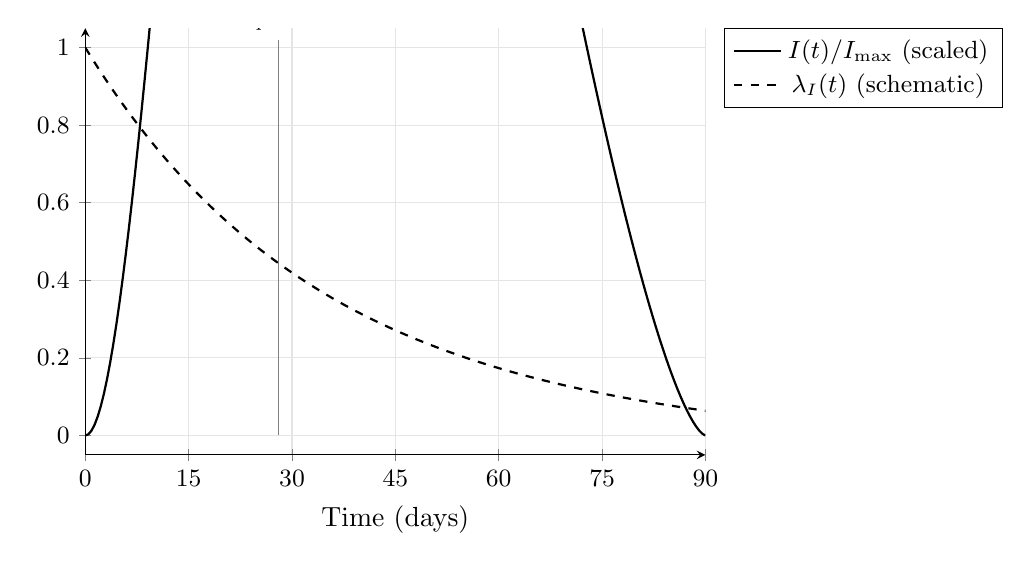
\begin{tikzpicture}
\begin{axis}[
  width=0.78\textwidth, height=7cm,
  xlabel={Time (days)},
  ylabel={},
  xmin=0, xmax=90,
  ymin=-0.05, ymax=1.05,
  grid=major, grid style={gray!20},
  legend pos=outer north east,
  legend style={font=\small},
  xtick={0,15,30,45,60,75,90},
  ytick={0,0.2,0.4,0.6,0.8,1.0},
  yticklabel style={font=\small},
  xticklabel style={font=\small},
  axis y line=left,
  axis x line=bottom,
]
%% I(t): rises to peak ~day 30, then falls (scaled to [0,1])
\addplot[thick, black, domain=0:90, samples=200]
  { max(0, 4*x^2 / (x^2 + 900) * (1 - x/90)^1.5 * 3.5 )};
\addlegendentry{$I(t)/I_{\max}$ (scaled)}

%% lambda_I(t): large near t=0, small near t=T, roughly exponential decay
\addplot[thick, black, dashed, domain=0:90, samples=200]
  {0.95*exp(-0.03*x) + 0.05*(1 - x/90)};
\addlegendentry{$\lambda_I(t)$ (schematic)}

%% Epidemic peak marker
\draw[black!50, thin] (axis cs:28, 0) -- (axis cs:28, 1.02);
\node[above, font=\scriptsize] at (axis cs:28, 1.02) {peak};

\end{axis}
\end{tikzpicture}
\caption{Schematic of $I(t)$ (solid, scaled to $[0,1]$) and the adjoint
         variable $\lambda_I(t)$ (dashed) for the SIR model.
         The adjoint variable is large near $t=0$, when a perturbation
         to the infectious compartment has the most time to affect the
         total burden $J = \int I\,dt$, and decays toward zero as
         $t \to T$.
         This gives $\lambda_I(t)$ a concrete interpretation as the
         marginal value of reducing the infectious population at time $t$:
         interventions are most cost-effective when $\lambda_I$ is large.}
\label{fig:sir_lambdaI}
\end{figure}

The adjoint variable $\lambda_I(t)$ has a concrete epidemiological
interpretation: it measures the marginal benefit of reducing the
infectious population at time $t$.
When $\lambda_I$ is large (early epidemic), reducing $I$ by one
person-day saves many future infections.
When $\lambda_I$ is small (late epidemic), most transmission has
already occurred, so the marginal benefit is low.
This interpretation is available from the adjoint computation alone,
with no additional work.

The terminal condition $\vec{\lambda}(T) = \vec{0}$ is not the same
as starting the forward ODE from initial condition $\vec{0}$ and running it
in reverse. The two problems have different structures: the forward
ODE is driven by $F(\vec{u}; \vec{p})$, while the adjoint ODE
is driven by $J_F^T \vec{\lambda}$ with a forcing term from $g$.
The backward direction comes from the integration by parts, not from
reversing time. The distinction matters for implementation: you run
\texttt{ode45} with \texttt{tspan = [T, 0]}, not with a negated vector field.

\unifyingidea{3} The adjoint variable $\lambda_I(t)$ illustrates Unifying Idea~3: local SA is a linearization.
The adjoint variable displays the
local sensitivity of $J$ throughout the simulation period.
This continuous record of sensitivity is the local SA analog of
what global SA asks globally: how does $J$ respond to perturbations
at each moment in time? Chapter~9 will ask the same question
for perturbations of the parameters across their full uncertainty
ranges rather than perturbations of the state at specific times.
The adjoint provides the linearization; global SA provides
the full nonlinear picture.

\unifyingidea{1} The sensitivity indices $\SI{p_i}{J}$ computed
in this chapter via the adjoint are exactly the normalized derivatives
of Unifying Idea~1 from Chapter~1: the ratio of relative changes in $J$ to relative
changes in each \POI $p_i$. The adjoint is simply a dramatically
more efficient algorithm for computing those same derivatives
when the model has many \POIs and few \QOIs.

\begin{selfcheck}
The adjoint variable $\lambda_R(t)$ for the recovered compartment
satisfies $-\dot{\lambda}_R = -\mu\lambda_R$ with $\lambda_R(T) = 0$.
(a) Solve this ODE analytically (backward from $T$).
(b) What does the solution tell you about the sensitivity of $J$
    to perturbations of the recovered compartment?
\end{selfcheck}
\begin{scAnswer}
(a) $-\dot{\lambda}_R = -\mu\lambda_R$ gives $\dot{\lambda}_R = \mu\lambda_R$
with $\lambda_R(T) = 0$.
Solution: $\lambda_R(t) = 0$ for all $t \in [0,T]$.
(The only solution to a linear ODE with zero terminal condition and
a coefficient that keeps it at zero is identically zero when the
equation has no forcing term.)

(b) $\lambda_R(t) = 0$ means that perturbations to $R(t)$ have no
effect on $J = \int I\,dt$. This makes biological sense: recovered
individuals do not contribute to future transmission (in the basic
SIR model without waning immunity), so changing $R(t)$ does not
change the integral of $I$.
\end{scAnswer}

%%------------------------------------------------------------
\section{Discrete vs.\ Continuous Adjoint}
\label{sec:discretecont}
%%------------------------------------------------------------

The adjoint ODE~\eqref{eq:adj_vec} is the \emph{continuous adjoint}:
it is derived by differentiating the continuous ODE and then discretizing
for numerical integration. An alternative is the \emph{discrete adjoint}:
discretize the ODE first and then adjoint the discrete system.
For linear ODEs with fixed step sizes, the two approaches give
identical results. For nonlinear ODEs with adaptive step-size control,
they can differ.

In practice: if your ODE solver uses fixed step sizes, either adjoint
is acceptable. If it uses adaptive step sizes (as \texttt{ode45} does),
the continuous adjoint requires storing the forward solution densely
enough to interpolate accurately, while the discrete adjoint requires
differentiating through the step-size controller.
For the SA computations in this book, the continuous adjoint with
dense output storage is the more practical approach.
Sirkes and Tziperman~\cite{sirkes1997finite} discuss these subtleties
for geophysical models. Smith~\cite{smith2014uncertainty} develops the
adjoint ODE formalism for general parameter-dependent dynamical systems
in \S9.4, with additional implementation guidance for systems with
stochastic forcing.

\medskip
\noindent\textbf{Neural ODEs.}
In 2018, Chen et al.~\cite{chen2018neural} demonstrated that
the adjoint calculation derived in this chapter can be used to train
certain deep neural networks. The network defines $\vec{F}(\vec{u};\theta)$
for parameters $\theta$; the loss function plays the role of $J$;
and the training algorithm integrates the adjoint ODE backward
to compute $\partial J/\partial\theta_i$ for all network parameters.
The phrase ``backpropagation through time,'' familiar from recurrent
neural networks, refers to the discrete version of this same
backward integration. The continuous limit is precisely the adjoint
ODE derived here.

%%------------------------------------------------------------
\section{MATLAB Laboratory: The SIR Adjoint in Practice}
\label{sec:ch6matlab}
%%------------------------------------------------------------

This laboratory implements the full forward-adjoint computation
for the SIR model and verifies the result against the FSE approach
from Chapter~4.

\textbf{Setup.}
Use the SIR model with \POIs $\vec{p} = (k, \beta, \tau, L)$,
nominal values $k=5$, $\beta=0.06$, $\tau=7$, $L=10{,}000$,
initial conditions $S_0=999$, $I_0=1$, $R_0=0$, $N=1000$,
and $T = 90$~days.
The response functional is $J = \int_0^{90} I(t)\,dt$.

\textbf{Part 1: Solve the forward SIR with dense output.}
Solve the SIR system using \texttt{ode45} with option
\texttt{'Refine', 8} or dense interpolation, storing the solution
on a fine uniform grid with spacing $\Delta t = 0.1$~days.
Store $(S, I, R)$ at every grid point; this array is needed
for the adjoint coefficient evaluation.

\medskip\noindent
\textbf{Interpolation (required before the backward solve).}
Before integrating the adjoint backward, build interpolants of
the forward solution so the adjoint ODE can evaluate $S(t)$,
$I(t)$, and $R(t)$ at any time during the backward pass:
\begin{verbatim}
S_fn = griddedInterpolant(t_fwd, U(:,1), 'pchip');
I_fn = griddedInterpolant(t_fwd, U(:,2), 'pchip');
R_fn = griddedInterpolant(t_fwd, U(:,3), 'pchip');
\end{verbatim}
Pass these interpolants into the adjoint function. Skipping this
step is the most common cause of errors in the adjoint lab.

\textbf{Part 2: Solve the adjoint system backward.}
Implement the adjoint ODEs~\eqref{eq:adj_S}--\eqref{eq:adj_R}.
Note that these depend on the forward solution $(S(t), I(t), R(t))$,
which must be interpolated from the stored grid.

\begin{verbatim}
function dlam = sir_adjoint(t, lam, S_fn, I_fn, R_fn, k, beta, tau, L)
%% Adjoint ODEs for SIR model
%% Integrate BACKWARD: call with tspan = [T, 0]

N     = 1000;
gamma = 1/tau;  mu = 1/L;
S = S_fn(t); I = I_fn(t); R = R_fn(t);   %% interpolate

lS = lam(1); lI = lam(2); lR = lam(3);

%% -d(lambda)/dt = J_F^T * lambda - grad_u(g)
%% Note: g = I, so grad_u(g) = (0, 1, 0)
dlam(1) = -(  (-k*beta*I/N - mu)*lS + (k*beta*I/N)*lI        );
dlam(2) = -(  (-k*beta*S/N)*lS + (k*beta*S/N - gamma - mu)*lI ...
              + gamma*lR - 1  );
dlam(3) = -(  -mu*lR                                          );

dlam = dlam(:);
end
\end{verbatim}

Solve from $t = T$ to $t = 0$ with terminal conditions
$\vec{\lambda}(T) = (0,0,0)$.

\textbf{Part 3: Plot $I(t)$ and $\lambda_I(t)$.}
On a single axis, plot the epidemic curve $I(t)$ (left scale)
and the adjoint variable $\lambda_I(t)$ (right scale).
Annotate the epidemic peak. Confirm that $\lambda_I$ is largest
near $t=0$ and smallest near $t=T$.

\textbf{Part 4: Compute sensitivities and produce a tornado plot.}
Evaluate the integrals~\eqref{eq:dJdbeta}--\eqref{eq:dJdL}
numerically using the trapezoidal rule. Normalize to obtain
$\SI{p_j}{J}$ for all four \POIs. Produce a tornado plot
and identify which parameter has the greatest influence on the
total disease burden.

\textbf{Part 5: Verify against Chapter 4 FSE results.}
From Chapter~4's MATLAB lab, retrieve the SI values computed by
the FSE at a single time point. Compare with the adjoint-based
SIs for $J = \int I\,dt$. Note: the two computations answer
\emph{different} questions (the FSE computes $\SI{p_j}{I(t)}$
at a fixed $t$, while the adjoint computes $\SI{p_j}{\int I\,dt}$),
so the numerical values will differ.
Instead, verify that $\SI{\beta}{J} = \SI{k}{J}$ to at least 4
significant figures (both should equal 1 for the SIR model with
this parameterization) and discuss whether the ratio holds exactly.

\textbf{Part 6: Timing comparison.}
Time the adjoint computation (Parts 1--4) against the FSE approach
from Chapter~4 (solve the 15-equation augmented system four times).
At what number of parameters $m$ would you expect the adjoint
to be faster? Does the timing crossover occur near $m = r = 1$
as the theory predicts?

%%------------------------------------------------------------
\section{Exercises}
%%------------------------------------------------------------

\begin{exercise}[\bloom{L3}]
\label{ex:ch6:scalar}
For the scalar ODE $\dot{u} = r u(1-u/K)$ (logistic) with
$J = \int_0^T u\,dt$ (total population over time):
\begin{enumerate}[label=(\alph*)]
  \item Write the adjoint ODE and terminal condition.
  \item Show that the adjoint ODE is linear in $\lambda(t)$
        even though the forward ODE is nonlinear in $u(t)$.
  \item Explain why the adjoint ODE depends on the forward solution $u(t)$.
  \item In MATLAB, solve the forward and adjoint ODEs simultaneously
        (forward from $0$ to $T$; store; then backward from $T$ to $0$)
        for $r=0.5$, $K=100$, $u_0=10$, $T=20$.
        Plot $u(t)$ and $\lambda(t)$.
\end{enumerate}
\end{exercise}

\begin{exercise}[\bloom{L3}]
\label{ex:ch6:IBP}
State in your own words what integration by parts accomplishes in
Step~3 of the Lagrange multiplier derivation, and why this is
analogous to the matrix transposition $A \to A^T$ in Chapter~5.
Then verify equation~\eqref{eq:IBP} directly by differentiating
the product $\lambda w$ and integrating over $[0,T]$.
\end{exercise}

\begin{exercise}[\bloom{L4}]
\label{ex:ch6:SIRfull}
Using your MATLAB implementation from the laboratory:
\begin{enumerate}[label=(\alph*)]
  \item Compute $\SI{\beta}{J}$, $\SI{k}{J}$, $\SI{\tau}{J}$,
        $\SI{L}{J}$ via the adjoint for $J = \int_0^{90} I\,dt$.
  \item Verify that $\SI{k}{J} = \SI{\beta}{J}$ to at least 6 significant
        figures. Explain this result using the structure of the SIR model.
  \item If you could implement one intervention that reduces a single
        parameter by $20\%$, which parameter would you target to most
        reduce the total disease burden? Justify using the tornado plot.
  \item Compare the computation time with the FSE approach from Chapter~4.
\end{enumerate}
\end{exercise}

\begin{exercise}[\bloom{L4}]
\label{ex:ch6:costtable}
Fill in the computation cost table for the SIR model with
$r=1$ response functional ($J = \int I\,dt$) and $n=3$ state variables:

\begin{center}
\begin{tabular}{lcc}
\toprule
$m$ (number of \POIs) & FSE cost (ODE solves) & Adjoint cost (ODE solves) \\
\midrule
4 & & \\
10 & & \\
50 & & \\
500 & & \\
\bottomrule
\end{tabular}
\end{center}

If each ODE solve takes 30~seconds, at what value of $m$ does the
adjoint become more than 10~times faster than the FSE?
\end{exercise}

\begin{exercise}[\bloom{L4}]
\label{ex:ch6:interpretation}
Explain in plain language, without any equations, why:
\begin{enumerate}[label=(\alph*)]
  \item The adjoint ODE must be integrated backward from $t=T$
        rather than forward from $t=0$.
  \item The adjoint variable $\lambda_I(t)$ for the SIR model
        and response $J = \int I\,dt$ is larger near $t=0$ than near $t=T$.
  \item A public health agency that wants to minimize total disease
        burden should focus interventions on the early phase of the
        epidemic, when $\lambda_I$ is large. Use $\lambda_I(t)$
        to quantify this recommendation.
  \item The terminal condition $\vec{\lambda}(T) = \vec{0}$ is
        not the same as running the forward ODE backward with initial
        condition $\vec{0}$.
\end{enumerate}
\end{exercise}

\begin{exercise}[\bloom{L5}]
\label{ex:ch6:SEIR}
Extend the SIR adjoint treatment to the SEIR model:
\begin{align*}
  \dot{S} &= \mu N - k\beta SI/N - \mu S, \\
  \dot{E} &= k\beta SI/N - (\nu + \mu)E, \\
  \dot{I} &= \nu E - (\gamma + \mu)I, \\
  \dot{R} &= \gamma I - \mu R,
\end{align*}
with \POIs $\vec{p} = (k, \beta, \tau_E, \tau_I, L)$
(interpretable parameterization: $\nu = 1/\tau_E$, $\gamma = 1/\tau_I$,
$\mu = 1/L$) and response functional $J = \int_0^T I(t)\,dt$.

Design the complete adjoint SA study, specifying:
\begin{enumerate}[label=(\alph*)]
  \item The $4\times4$ Jacobian $J_F$ at a generic point
        $(S, E, I, R)$.
  \item All four adjoint ODEs and their terminal conditions.
  \item The sensitivity formulas $dJ/dp_j$ for all five \POIs.
  \item The MATLAB implementation strategy (how you would store
        the forward solution and integrate the adjoint backward).
  \item What additional cost the SEIR adjoint requires compared
        to the SIR adjoint (in terms of ODE solves and storage).
\end{enumerate}
\end{exercise}

\begin{exercise}[\bloom{L6}]
\label{ex:ch6:disagreement}
A climate modeler reports: ``We implemented the adjoint to compute
sensitivities for our model with 200 parameters, but the results
disagree with forward sensitivity analysis by approximately $15\%$
for some parameters. The adjoint must have a bug.''

Identify three distinct causes that could produce this discrepancy
without any coding error. For each cause:
\begin{enumerate}[label=(\alph*)]
  \item State the cause precisely.
  \item Describe a diagnostic test that would confirm or rule it out.
  \item Describe the correction if the cause is confirmed.
\end{enumerate}
\end{exercise}

%%------------------------------------------------------------

